\documentclass[a4paper, 12pt]{article}

\usepackage{geometry}
\usepackage{tikz}
    \usetikzlibrary{patterns,decorations.pathreplacing,snakes,arrows.meta}
    \tikzset{box/.style={draw, thick, minimum width=1cm, minimum height=1cm}}
\usepackage{bigints}
\usepackage{tabularx}
\usepackage{fancyhdr}
\usepackage{amsfonts}
\usepackage{graphicx}
\usepackage{fontenc}
\usepackage{amssymb}
\usepackage{amsmath}
\usepackage{multicol}
\usepackage{enumitem}
%\usepackage{wrapfig}
\usepackage{longtable}
\usepackage{array}
\usepackage{bm}
\usepackage{color}
\usepackage{textcomp}
\setlength{\multicolsep}{5.0pt plus 2.0pt minus 1.5pt}% 50% of original values
\geometry{a4paper, portrait, top=2.5cm, left=2.5cm, right=2.5cm, bottom=2.5cm}

\tolerance=1
\emergencystretch=\maxdimen
\hyphenpenalty=10000
\hbadness=10000

\newcommand{\R}{\mathbb{R}}
\newcommand{\Z}{\mathbb{Z}}
\newcommand{\C}{\mathbb{C}}
\newcommand{\N}{\mathbb{N}}
\newcommand{\Q}{\mathbb{Q}}


\renewcommand{\baselinestretch}{1.2}
\newcounter{choice}
\renewcommand\thechoice{\alph{choice}}
\newcommand\choicelabel{\thechoice.}

\newenvironment{choices}%
{\list{\choicelabel}%
	{\usecounter{choice}\def\makelabel##1{\hspace{0.3cm}\llap{##1}}%
		\settowidth{\leftmargin}{\hskip\labelsep\hskip 0em}%
		\def\choice{%
			\item
		} % choice
		\labelwidth\leftmargin\advance\labelwidth-\labelsep
		\topsep=0pt
		\partopsep=0pt
	}%
}%
{\endlist}

\newenvironment{oneparchoices}%
{%
	\setcounter{choice}{0}%
	\def\choice{%
		\refstepcounter{choice}%
		\ifnum\value{choice}>1\relax
		\penalty -50\hskip 2cm plus 1em
		\fi
		\choicelabel
		\nobreak\enskip
	}% choice
	% If we're continuing the paragraph containing the question,
	% then leave a bit of space before the first choice:
	\ifvmode\else\enskip\fi
	\ignorespaces
}%
{}
\tolerance=1
\emergencystretch=\maxdimen
\hyphenpenalty=10000
\hbadness=10000

\fancyfoot[L]{\textit{5002221132}}
\fancyfoot[R]{\textit{Tetew}}
\renewcommand{\headrulewidth}{0pt}
\renewcommand{\footrulewidth}{2pt}
\pagestyle{fancy}
\pagenumbering{gobble}
\begin{document}
\begin{center}
    \large{TES BAGIAN PERTAMA}\\
    Bentuk Soal: Isian Singkat\\
    Waktu: 60 menit\\
    ~
\end{center}
\textbf{SOAL}
\begin{enumerate}
    \item Misalkan $\theta_n=\arctan{n}$. Nilai dari $\lim\limits_{n\rightarrow\infty}(\theta_{n+1}-\theta_n)$ adalah \dots
    \item Diberikan $\mathbb{Z}_3[x]/I$ dengan $I$ adalah ideal yang dibangun oleh $x^4+x+2$, invers dari $x^2+x+I \in \mathbb{Z}_3[x]/I$ adalah \dots
    \item Jika $K$ dan $L$ dua subruang dari $\mathbb{R}^{10}$ dan untuk dim $K$ + dim $L$ = 12, maka nilai terkecil yang mungkin untuk dim$(K \cap L)$ adalah \dots
    \item Misalkan $v$ dan $w$ adalah akar-akar yang berbeda yang dipilih secara acak dari persamaan $z^{2024}-1=0$. Misalkan $\frac{m}{n}$ adalah probabilitas dari $\sqrt{2+\sqrt{3}}\leq\left|v+w\right|$, di mana $m$ dan $n$ adalah bilangan bulat positif yang relatif prima, nilai dari $m+n$ adalah $\dots$
    \item Enam orang siswa akan duduk pada tiga meja bundar, dimana setiap meja akan diduduki oleh minimal satu siswa. Banyaknya cara untuk melakukan hal tersebut adalah \dots
\end{enumerate}
\textbf{\underline{SOLUSI}}
\begin{enumerate}
    \item Karena $\displaystyle\lim_{n\to\infty}\arctan{n}=\dfrac{\pi}{2}$ dan $\displaystyle\lim_{n\to\infty}\theta_n=\lim_{n\to\infty}\theta_{n+1}$, maka 
    \[\lim_{n\to\infty}(\theta_{n+1}-\theta_n)=\dfrac{\pi}{2}-\dfrac{\pi}{2}=\boxed{0}\]

    \item Misalkan $\bm{p}(x)=x^4+x+2$ dan $ax^3+bx^2+cx+d+I$ (pangkat tertinggi di ring kuasi) adalah invers dari $x^2+x+I$. Maka
    \begin{align*}
        (ax^3+bx^2+cx+d+I)(x^2+x+I)=&1+I\\
        ax^5+(a+b)x^4+(b+c)x^3+(c+d)x^2+dx=&1+I\\
        \cline{1-2}
        (a+b)x^4+(b+c)x^3+(c+d-a)x^2+(d-2a)x=&1+I&\color{red}-ax\cdot \bm{p}(x)\\
        \cline{1-2}
        (b+c)x^3+(c+d-a)x^2+(d-b)x-2(a+b)=&1+I&\color{red}-(a+b)\cdot \bm{p}(x)\\
    \end{align*}
    Kemudian didapatkan sistem persamaan linear 
    \begin{align*}
        b+c=&0\\
        c+d-a=&0\\
        d-b=&0\\
        a+b=&1
    \end{align*}
    Dapat dicek bahwa solusinya adalah $a=0,\,b=1,c=2,d=1$. Sehingga invers dari $x^2+x+I$ adalah $\boxed{x^2+2x+1+I}$.

    \item Karena $K$ dan $L$ adalah subruang dari $\R^{10}$, maka $K+L$ juga merupakan subruang dari $\R^{10}$. Selanjutnya diketahui hubungan
    \[\dim(K+L)=\dim(K)+\dim(L)-\dim(K\cap L)\]
    Dan juga karena $K+L$ adalah subruang berakibat $\dim(K+L)\leq 10$ atau
    \begin{align*}
        \dim(K)+\dim(L)-\dim(K\cap L)\leq 10\\
        12-\dim(K\cap L)\leq 10\\
        \dim(K\cap L)\geq 2
    \end{align*}
    Jadi nilai terkecil yang mungkin untuk $\dim(K\cap L)$ adalah $\boxed{2}$.

    \item Misalkan $v=\cos\theta_1+i\sin\theta_1$ dan $w=\cos\theta_2+i\sin\theta_2$. Selanjutnya $|v+w|$ dapat ditulis sebagai berikut
    \begin{align*}
        |v+w|&=\sqrt{(\cos\theta_1+\cos\theta_2)^2+(\sin\theta_1+\sin\theta_2)^2}\\
        &=\sqrt{\cos^2\theta_1+\cos^2\theta_2+2\cos\theta_1\cos\theta_2+\sin^2\theta_1+\sin^2\theta_2+2\sin\theta_1\sin\theta_2}\\\
        &=\sqrt{2+2(\cos\theta_1\cos\theta_2+\sin\theta_1\sin\theta_2)}\\
        &=\sqrt{2+2\cos(\theta_1-\theta_2)}
    \end{align*}
    Ingat bahwa $\theta_1,\theta_2\in\left\{\left.\dfrac{\pi k}{1012}\right|k=\{0,1,\dots,2023\}\right\}$ yang berakibat $\theta_1-\theta_2$ dapat ditulis sebagai $\dfrac{\pi k}{1012}$ untuk suatu $k\in\{0,1,\dots,2023\}$.
    \begin{align*}
        |v+w|\geq \sqrt{2+\sqrt{3}}\\
        \sqrt{2+2\cos(\theta_1-\theta_2)}\geq \sqrt{2+\sqrt{3}}\\
        2\cos\left(\dfrac{\pi k}{1012}\right)\geq \sqrt{3}\\
        -\dfrac{\pi}{6}\leq \dfrac{\pi k}{1012} \leq \frac{\pi}{6}\\
        -168\frac{2}{3}\leq k\leq 168\frac{2}{3}
    \end{align*}
    Karena $k$ bulat maka $k\in\{-168,-167,\dots,168\}$ yang dimana memiliki 337 kemungkinan. Dengan demikian probabilitasnya adalah $\dfrac{337}{2024}$. Selanjutnya dapat dicek bahwa $\gcd(337,2024)=1$, sehingga $m+n=337+2024=\boxed{2361}$.
    \item Permasalahan diatas dapat direpresentasikan sebagai banyaknya pasangan $(x_1,x_2,x_3)$ yang memenuhi
    \begin{align*}
        x_1+x_2+x_3=6\quad
        x_1,x_2,x_3\geq 1
    \end{align*}
    misalkan $y_1=6-x_1$, $y_2=6-x_2$, dan $y_3=6-x_3$. Maka permasalahan diatas dapat direpresentasikan sebagai banyaknya pasangan $(y_1,y_2,y_3)$ yang memenuhi
    \begin{align*}
        y_1+y_2+y_3=3\quad
        y_1,y_2,y_3\geq 0
    \end{align*}
    Dengan demikian dengan metode \textit{stars and bars} didapatkan banyaknya cara enam siswa duduk adalah $\displaystyle\binom{5}{3}=\boxed{6}$.
\end{enumerate}
\newpage
\begin{center}
    \large{TES BAGIAN KEDUA}\\
    Bentuk Soal: Uraian\\
    Waktu: 120 menit
\end{center}
\textbf{SOAL}
\begin{enumerate}
  \item Diberikan barisan bilangan positif $(a_n)_{n\geq 1}$ sedemikian hingga
    $$a_{n+1}\leq a_{n}+\dfrac{1}{(n+1)^2}$$
    untuk setiap $n\geq 1$. Buktikan bahwa $(a_n)_{n\geq 1}$ merupakan barisan konvergen.
    \item Diberikan homomorfisma ring $f:\mathbb{Z}[x]\to \mathbb{Z}_2[x]$ dengan 
    \begin{align*}
        f(a_0+a_1x+\cdots +a_nx^n) := \overline{a_0}+\overline{a_1}x+\cdots + \overline{a_n}x^n,
    \end{align*}
    dan $\overline{a_i}=a_i\mod 2$ untuk setiap $i=0,1,2,\dots,n$. 
    \begin{enumerate}
        \item Tentukan $\ker f$
        \item Tunjukkan bahwa $\ker f$ adalah ideal prima di $\mathbb{Z}[x]$
    \end{enumerate}
    \item Diberikan suatu ruang vektor berdimensi hingga $V$ serta subruang $K$ dan $L$ dari $V$. Didefinisikan
    $$W=K+L=\{k+l\mid k\in K, l\in L\}.$$
    Buktikan bahwa
    \begin{enumerate}
        \item $K\cap L$ dan $W$ merupakan subruang dari $V$
        \item $\dim(W) = \dim(K) + \dim(L)-\dim(K\cap L)$.
    \end{enumerate}
    \item Diberikan fungsi kompleks $f(z)=u(x,y)+iv(x,y)$ merupakan fungsi analitik dan memenuhi $u(x,y)\leq x$ untuk semua $z=x+iy\in \mathbb{C}$. Tunjukkan bahwa $f$ adalah polinomial kompleks berderajat 2.
    \item Diberikan bilangan bulat tak negatif $k$ dan $n$ sehingga $0 \leq k <n$. Berikan bukti kombinatorial bahwa 
	\begin{equation*}
	\displaystyle\sum_{j=0}^{k} \left( \begin{array}{c}
	n\\j
	\end{array} \right) = \sum_{j=0}^{k} \left( \begin{array}{c}
	n-1-j\\k-j
	\end{array} \right)2^j
	\end{equation*}
\end{enumerate}
\textbf{\underline{SOLUSI}}
\begin{enumerate}
    \item Definisikan barisan $\displaystyle b_n=a_n+\sum_{k=n+1}^{\infty}\dfrac{1}{k^2}$. Sehingga 
    \[b_{n+1}-b_n=\left(a_{n+1}+\sum_{k=n+2}^{\infty}\dfrac{1}{k^2}\right)-\left(a_n+\sum_{k=n+1}^{\infty}\dfrac{1}{k^2}\right)=a_{n+1}-a_{n}-\frac{1}{(n+1)^2}\leq 0\]
    yang berarti $b_{n+1}\leq b_n$ untuk setiap $n\geq 1$. Dengan demikian barisan $b_n$ adalah barisan monoton tidak naik (turun atau konstan).

    Selanjutnya perhatikan bahwa $b_n> 0$ untuk setiap $n\geq 1$ karena $a_n$ adalah bilangan positif. Disisi lain juga
    \[b_n\leq a_0+\sum_{k=1}^{\infty}\dfrac{1}{k^2}=\dfrac{\pi^2}{6}+a_0\]
    Dengan demikian barisan $b_n$ adalah barisan terbatas. Sehingga dapat disimpulkan bahwa barisan $b_n$ konvergen (misalkan $b_n\to L\in\R$).

    Menggunakan sifat limit, maka
    \begin{align*}
        \lim_{n\to\infty}a_n&=\lim_{n\to\infty}\left(b_n-\sum_{k=n+1}^{\infty}\dfrac{1}{k^2}\right)\\
        &=L-\lim_{n\to\infty}\sum_{k=n+1}^{\infty}\dfrac{1}{k^2}=L-0=L
    \end{align*}
    Jadi barisan $(a_n)_{n\geq 1}$ juga barisan konvergen.
    \item \begin{enumerate}
        \item Secara definisi dapat ditulis sebagai
        \begin{align*}
            \ker f=\{p(x)\in\Z[x]\mid f(p(x))=0\}
        \end{align*}
        Sehingga untuk $p(x)=a_0+a_1x+\cdots+a_nx^n$ dapat kita tinjau
        \begin{align*}
            f(p(x))&=0\\
            f\left(a_0+a_1x+\cdots+a_nx^n\right)&=0 \mod 2\\
            \overline{a_0}+\overline{a_1}X+\cdots + \overline{a_n}x^n&=0 \mod 2\\
            \overline{a_0}=\overline{a_1}=\cdots=\overline{a_n}&=0\mod 2
        \end{align*}
        Artinya anggota dari $\ker f$ adalah polinomial dengan koefisien genap semua. Atau dapat juga ditulis 
        \[\ker f=\left\{p(x)\in\Z[x]\mid p(x)=2q(x),\,q(x)\in\Z[x]\right\}\] 
        \item  Misalkan $r(x)=a_0+a_1+\dots+a_n\in\ker f$ dan $s(x)=b_0+b_1+\dots+b_n\in\ker f$, maka $f(r(x))=0$ dan $f(s(x))=0$. Sehingga kita punya
        \begin{itemize}
            \item $f(r(x)-s(x))=f(r(x))-f(s(x))=0+0=0$ yang berarti $r(x)-s(x)\in\ker f$.
            \item Misalkan $u(x)=r(x)s(x)=c_0+c_1+\dots+c_n$ dengan $c_k=\sum_{i=0}^{k}a_kb_{k-i}$ untuk $k=0,1,\dots,n$. Karena $a_i$ dan $b_i$ adalah bilangan genap, maka penjumlahan dan perkaliannya yaitu $c_k$ juga bilangan genap untuk setiap $k=0,1,\dots,n$. Sehingga
            \[f(u(x))=f(r(x)s(x))=\overline{c_0}+\overline{c_1}x+\cdots+\overline{c_n}x^n=0\]
            Jadi $r(x)s(x)\in\ker f$.
        \end{itemize}
        Dengan demikian $\ker f$ merupakan subring dari $\Z[x]$.

        Selanjutnya kita misalkan ulang $r(x)s(x)\in\ker f$ namun $r(x)\notin\ker f$ dan $s(x)\notin\ker f$, artinya terdapat koefisien $a_i$ dan $b_j$ yang ganjil. Hal ini berakibat bahwa $c_k \not\equiv 0 \mod 2$ untuk suatu $k\in\{0,1,\dots,n\}$. Hal ini berarti $f(u(x))=f(r(x)s(x))\ne 0$, yang bertentangan dengan asumsi bahwa $r(x)s(x)\in\ker f$. Dengan demikian haruslah $r(x)\in\ker f$ atau $s(x)\in\ker f$.

        $\therefore$ Terbukti bahwa $\ker f$ adalah ideal prima di $\Z[x]$.
    \end{enumerate}
    \item \begin{enumerate}
        \item 
    \end{enumerate}
    \item Fungsi $f$ analitik di $\C$ berarti $f$ dapat diekspansi sebagai deret berikut
    \begin{align*}
        f(z)=\sum_{n=0}^{\infty}a_nz^n
    \end{align*}
    
    \item Misalkan $S$ adalah himpunan yang mempunyai $n$ elemen yaitu $S=\{1,2,\dots,n\}$. Bagaimana total cara memilih maksimal $k$ elemen dari $S$?
    \begin{enumerate}[leftmargin=1.3cm]
        \item[\textbf{LHS}:] Untuk memilih $j=0,1,\dots$ elemen dari $S$ dapat dilakukan dengan $\binom{n}{j}$ cara. Selanjutnya total cara untuk memilih minimal 0 elemen dan maksimal $k$ elemen adalah
        \begin{align*}
            \sum_{j=0}^{k}\binom{n}{j}
        \end{align*}
        \item[\textbf{RHS}:] Andaikan kita memilih suatu elemen berurutan, sebut saja \textit{pivot} yang dimana {\color{red} elemen tersebut tidak akan dipilih}. 
        \begin{itemize}
            \item Untuk $j=0$, maka kita pilih elemen $1$ sebagai \textit{pivot}
            \begin{center}
                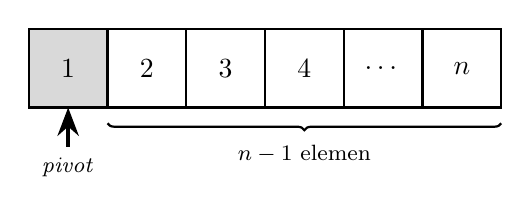
\begin{tikzpicture}
                    \foreach \i[count=\n] in {1,2,3,4,\dots,n}{
                        \ifnum\n=1
                            \node[box,fill=gray!30] at (\n,1.5){$\i$};
                        \else
                            \node[box] at (\n,1.5){$\i$};
                        \fi
                        }
                        \draw [thick,decoration={brace, mirror, raise=0.4cm},decorate] (1.5,1.2) -- (6.5,1.2) 
                        node [pos=0.5,anchor=north,yshift=-0.55cm] {\footnotesize $n-1$ elemen}; 

                        \draw[arrows = {-Stealth[reversed, reversed]},ultra thick] (1,0.5) node [below] {\footnotesize \textit{pivot}}-- (1,1);
                \end{tikzpicture}
            \end{center}
            Karena tersisa $n-1$ elemen, maka cara memilih $k$ elemen adalah \[\binom{n-1}{k}\]
            \item Untuk $j=1$, maka kita pilih elemen $2$ sebagai \textit{pivot}
            \begin{center}
                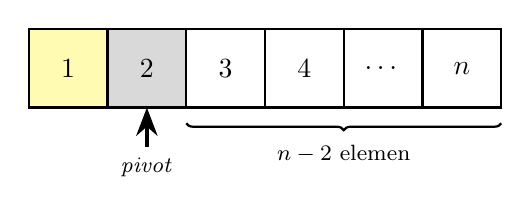
\begin{tikzpicture}
                    \foreach \i[count=\n] in {1,2,3,4,\dots,n}{
                        \ifnum\n<2
                            \node[box,fill=yellow!30] at (\n,1.5){$\i$};
                        \else
                            \ifnum\n=2
                                \node[box,fill=gray!30] at (\n,1.5){$\i$};
                            \else
                                \node[box] at (\n,1.5){$\i$};
                            \fi
                        \fi
                        }
                        \draw [thick,decoration={brace, mirror, raise=0.4cm},decorate] (2.5,1.2) -- (6.5,1.2) 
                        node [pos=0.5,anchor=north,yshift=-0.55cm] {\footnotesize $n-2$ elemen}; 

                        \draw[arrows = {-Stealth[reversed, reversed]},ultra thick] (2,0.5) node [below] {\footnotesize \textit{pivot}}-- (2,1);
                \end{tikzpicture}
            \end{center}
            Selanjutnya kita akan memilih $k-1$ elemen dari $n-2$ elemen terlebih dahulu. Kemudian karena maksimal adalah $k$ elemen, maka kita punya pilihan untuk memilih elemen $1$ sebagai elemen ke-$k$ atau tidak (2 kemungkinan). Sehingga total cara adalah \[\binom{n-2}{k-1}\cdot 2\]
            \item Untuk $j=2$, maka kita pilih elemen $3$ sebagai \textit{pivot}
            \begin{center}
                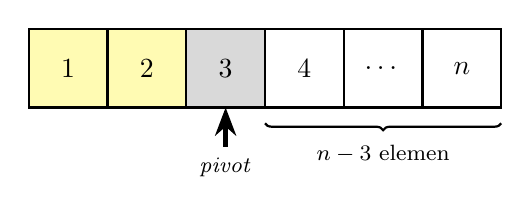
\begin{tikzpicture}
                    \foreach \i[count=\n] in {1,2,3,4,\dots,n}{
                        \ifnum\n<3
                            \node[box,fill=yellow!30] at (\n,1.5){$\i$};
                        \else
                            \ifnum\n=3
                                \node[box,fill=gray!30] at (\n,1.5){$\i$};
                            \else
                                \node[box] at (\n,1.5){$\i$};
                            \fi
                        \fi
                        }
                        \draw [thick,decoration={brace, mirror, raise=0.4cm},decorate] (3.5,1.2) -- (6.5,1.2) 
                        node [pos=0.5,anchor=north,yshift=-0.55cm] {\footnotesize $n-3$ elemen}; 

                        \draw[arrows = {-Stealth[reversed, reversed]},ultra thick] (3,0.5) node [below] {\footnotesize \textit{pivot}}-- (3,1);
                \end{tikzpicture}
            \end{center}
            Analog kita memilih $k-2$ elemen dari $n-3$ dan mempertimbangkan masing-masing elemen $1$ dan $2$ sebagai elemen ke-$(k-1)$ dan ke-$k$ atau tidak ($2^2$ kemungkinan). Sehingga total cara adalah \[\binom{n-3}{k-2}\cdot 2^2\]
            \[\vdots\]
            \item Secara umum untuk elemen ke-$j$, maka elemen \textit{pivot}-nya adalah $j+1$
            \begin{center}
                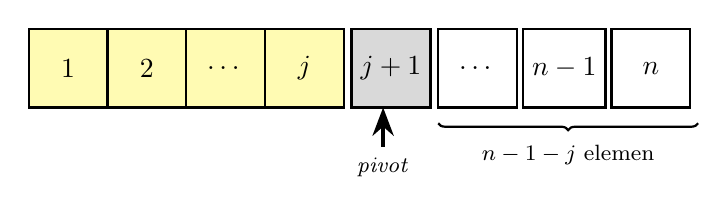
\begin{tikzpicture}
                    \foreach \i[count=\n] in {1,2,\dots,j,j+1,\dots,n-1,n}{
                        \ifnum\n<5
                            \node[box,fill=yellow!30] at (\n,1.5){$\i$};
                        \else
                            \ifnum\n=5
                                \node[box,fill=gray!30] at ({\n+.1*(\n-4)},1.5){$\i$};
                            \else
                                \node[box] at ({\n+.1*(\n-4)},1.5){$\i$};
                            \fi
                        \fi
                        }
                        \draw [thick,decoration={brace, mirror, raise=0.4cm},decorate] (5.7,1.2) -- (9,1.2) 
                        node [pos=0.5,anchor=north,yshift=-0.55cm] {\footnotesize $n-1-j$ elemen}; 

                        \draw[arrows = {-Stealth[reversed, reversed]},ultra thick] (5,0.5) node [below] {\footnotesize \textit{pivot}}-- (5,1);
                \end{tikzpicture}
            \end{center}
            Terdapat $k-j$ elemen yang harus dipilih dari $n-1-j$ elemen dan masing-masing $j$ elemen memiliki 2 kemungkinan untuk dipilih atau tidak ($2^j$ kemungkinan). Sehingga total cara adalah \[\binom{n-1-j}{k-j}\cdot 2^j\]
        \end{itemize}
        Dengan cara diatas, maka total cara untuk memilih maksimal $k$ elemen dari $S$ adalah
        \begin{align*}
            \sum_{j=0}^{k}\binom{n-1-j}{k-j}\cdot 2^j
        \end{align*}
    \end{enumerate}
    $\therefore$ \textbf{LHS $=$ RHS} sehingga pernyataan tersebut benar.
\end{enumerate}
\end{document}